\documentclass[11pt, a4paper]{article}

% Fonts and Encoding
\usepackage[utf8]{inputenc}
\usepackage[T1]{fontenc}

% Math and Symbols
\usepackage{amsmath, amssymb, amsthm, amsfonts, mathrsfs, mathtools}

% Layout and Geometry
\usepackage{geometry}
\geometry{a4paper, margin=1in}

% Formatting and Graphics
\usepackage{graphicx, xcolor, enumitem, booktabs, array, tabularx}

% TikZ for Illustrations
\usepackage{tikz}
\usetikzlibrary{arrows.meta, positioning, shapes.geometric, calc, backgrounds, matrix}

% Clickable Links and TOC
\usepackage{hyperref}
\hypersetup{
    colorlinks=true,
    linkcolor=blue,
    filecolor=magenta,      
    urlcolor=cyan,
    pdftitle={Advanced Mathematics Topic},
}

% Theorem Environments
\newtheorem{theorem}{Theorem}[section]
\newtheorem{lemma}[theorem]{Lemma}
\newtheorem{proposition}[theorem]{Proposition}
\newtheorem{corollary}[theorem]{Corollary}
\theoremstyle{definition}
\newtheorem{definition}{Definition}[section]
\newtheorem{axiom}{Axiom}[section]
\newtheorem{example}{Example}[section]
\theoremstyle{remark}
\newtheorem{remark}{Remark}[section]

% Custom Commands (Enforced standard notation)
\newcommand{\R}{\mathbb{R}}
\newcommand{\N}{\mathbb{N}}
\newcommand{\Z}{\mathbb{Z}}
\newcommand{\Q}{\mathbb{Q}}
\newcommand{\E}{\mathbb{E}}
\newcommand{\Prob}{\mathbb{P}}
\newcommand{\F}{\mathcal{F}}

\title{The Beta Probability Distribution: \\ Measure-Theoretic Foundations and Advanced Applications \\ \large Rigorous Practice Problem Set}
\author{Tashfeen Omran}
\date{\today}

\begin{document}

\maketitle
\tableofcontents
\newpage

\section{Concept Checklist \& Question Mapping}

To ensure comprehensive coverage of the theoretical concepts, logical structures, and proof techniques detailed in the foundational text, the following checklist maps each core concept to its corresponding problems in the practice set.

\renewcommand{\arraystretch}{1.5}
\noindent
\begin{tabularx}{\textwidth}{l X l}
\toprule
\textbf{ID} & \textbf{Theoretical Concept / Proof Technique} & \textbf{Problem Numbers} \\
\midrule
C1 & Density Normalization \& The Kernel Method & 1, 2, 3 \\
C2 & Direct Measure Computation \& Borel Set Integration & 4, 5, 6 \\
C3 & Transformations \& Expectations (LOTUS) & 7, 8, 9, 10 \\
C4 & Theoretical Parameter Proofs \& Gamma Recursion & 11, 12, 13, 14 \\
C5 & The Four-Parameter (Generalized) Beta Distribution & 15, 16, 17 \\
C6 & Bayesian Inference, Conjugacy, \& Posterior Updating & 18, 19, 20 \\
C7 & Advanced Applications: ML \& Algorithmic Trading & 21, 22, 23 \\
C8 & Measure-Theoretic Limits \& Asymptotic Behavior & 24, 25 \\
C9 & Diagnostic Testing: "Find the Flaw" (Logic/Syntax) & 26, 27, 28, 29, 30 \\
\bottomrule
\end{tabularx}
\vspace{1em}

\section{Problem Set}

\subsection{Density Normalization and The Kernel Method}
\begin{enumerate}[label=\textbf{\arabic*.}]
    \item Let $Y$ be a continuous random variable representing the proportion of impurities in a chemical batch. Its probability density function is given by $f(y) = k y^4 (1-y)^3$ for $y \in [0, 1]$, and $0$ elsewhere. Using the Kernel Method, determine the exact value of the normalizing constant $k$.
    \item Prove that the Beta function is symmetric; that is, establish the logical equivalence $B(\alpha, \beta) = B(\beta, \alpha)$ using a rigorous change-of-variable integration technique.
    \item A random variable $X$ has a density proportional to $x^{2.5} (1-x)^{1.5}$ on the support $[0, 1]$. Express its normalizing constant strictly in terms of the Gamma function, $\Gamma(z)$.
\end{enumerate}

\subsection{Direct Measure Computation}
\begin{enumerate}[label=\textbf{\arabic*.}, resume]
    \item Let $Y \sim \text{Beta}(2, 2)$. Compute the exact probability measure of the Borel set $B = [0.25, 0.75]$.
    \item Prove that if $Y \sim \text{Beta}(1, 1)$, the probability measure reduces to the standard Uniform distribution, and compute $\Prob(Y \le y)$ for $y \in [0, 1]$.
    \item Let $Y \sim \text{Beta}(3, 1)$. Find the probability that $Y > 0.5$ via direct polynomial integration.
\end{enumerate}

\subsection{Transformations and Expectations (LOTUS)}
\begin{enumerate}[label=\textbf{\arabic*.}, resume]
    \item The proportion of time a machine is operational is modeled as $Y \sim \text{Beta}(2, 3)$. The weekly profit function is given by the polynomial $P(Y) = 50 + 100Y - 20Y^2$. Calculate the expected profit $\E[P(Y)]$ using the Law of the Unconscious Statistician (LOTUS) and the linearity of expectation.
    \item For the same machine in Problem 7, compute the variance of the profit, $\text{Var}(P(Y))$.
    \item Let $Y \sim \text{Beta}(\alpha, \beta)$. Derive the general formula for the $k$-th raw moment, $\E[Y^k]$, using the Gamma recursion trick.
    \item Find a counterexample to the claim that $\E[1/Y] = 1/\E[Y]$ by explicitly computing $\E[1/Y]$ for $Y \sim \text{Beta}(3, 2)$.
\end{enumerate}

\subsection{Theoretical Parameter Proofs}
\begin{enumerate}[label=\textbf{\arabic*.}, resume]
    \item Rigorously prove that the variance of $Y \sim \text{Beta}(\alpha, \beta)$ is given by $\sigma^2 = \frac{\alpha\beta}{(\alpha+\beta)^2(\alpha+\beta+1)}$.
    \item Prove that for $\alpha > 1$ and $\beta > 1$, the mode of the Beta distribution is uniquely located at $y_{\text{mode}} = \frac{\alpha-1}{\alpha+\beta-2}$.
    \item Establish the logical equivalence between the Incomplete Beta Function $I_y(\alpha, \beta)$ and the cumulative distribution function of a Binomial random variable when $\alpha$ and $\beta$ are integers.
    \item Prove that if $Y \sim \text{Beta}(\alpha, \beta)$, then the transformed variable $X = 1 - Y$ follows a $\text{Beta}(\beta, \alpha)$ distribution.
\end{enumerate}

\subsection{The Four-Parameter (Generalized) Beta Distribution}
\begin{enumerate}[label=\textbf{\arabic*.}, resume]
    \item Let $X$ follow a Generalized Beta distribution on the interval $[c, d]$ with shape parameters $\alpha$ and $\beta$. Derive the expected value $\E[X]$.
    \item Derive the variance $\text{Var}(X)$ for the Generalized Beta distribution defined in Problem 15.
    \item In project management (PERT analysis), a task's duration $X$ is bounded between $c = 5$ days and $d = 15$ days. If $X$ follows a Generalized Beta distribution with $\alpha = 4$ and $\beta = 4$, compute the exact probability that the task takes more than 10 days.
\end{enumerate}

\subsection{Bayesian Inference and Machine Learning}
\begin{enumerate}[label=\textbf{\arabic*.}, resume]
    \item Prove that the Beta distribution is the conjugate prior for the Bernoulli likelihood function.
    \item A Machine Learning model predicts the Click-Through Rate (CTR) $\theta$ of an ad. The prior is $\theta \sim \text{Beta}(2, 2)$. After observing 10 clicks out of 50 impressions, derive the posterior distribution $\pi(\theta \mid S)$.
    \item For the posterior distribution found in Problem 19, compute the Bayesian Maximum A Posteriori (MAP) estimate for the CTR.
\end{enumerate}

\subsection{Advanced Applications and Asymptotics}
\begin{enumerate}[label=\textbf{\arabic*.}, resume]
    \item \textbf{Thompson Sampling:} An AI agent evaluates two slot machines. Machine A has a posterior belief state $\theta_A \sim \text{Beta}(3, 1)$ and Machine B has $\theta_B \sim \text{Beta}(1, 3)$. Formulate the exact double integral required to compute $\Prob(\theta_A > \theta_B)$.
    \item \textbf{Algorithmic Trading:} The recovery rate $R$ of a defaulted bond is modeled as $R \sim \text{Beta}(2, 2)$. A credit derivative pays out $V = 100 \times \max(R - 0.5, 0)$. Compute the expected payout $\E[V]$.
    \item \textbf{Measure-Theoretic Limit:} Prove that as $\alpha \to \infty$ and $\beta \to \infty$ such that $\alpha = \beta$, the Beta probability measure converges weakly to a Dirac measure concentrated at $y = 0.5$.
    \item \textbf{Non-linear Transformation:} Let $Y \sim \text{Beta}(\alpha, 1)$. Derive the probability density function of the random variable $W = -\ln(Y)$ and identify its standard distribution family.
    \item \textbf{Product of Random Variables:} Let $Y_1, Y_2 \sim \text{Beta}(1, 1)$ be independent random variables. Derive the probability density function of their product, $Z = Y_1 Y_2$.
\end{enumerate}

\subsection{Advanced Diagnostic Testing: "Find the Flaw"}
\begin{enumerate}[label=\textbf{\arabic*.}, resume]
    \item \textbf{Find the Flaw:} "Let $Y \sim \text{Beta}(3, 3)$. To find $\E[Y^2]$, we compute $(\E[Y])^2 = (0.5)^2 = 0.25$." Identify the logical fallacy and compute the correct value.
    \item \textbf{Find the Flaw:} "Let $Y \sim \text{Beta}(4, 2)$. The normalizing constant is $\frac{\Gamma(4+2)}{\Gamma(4)\Gamma(2)} = \frac{6!}{4!2!} = 15$." Identify the mathematical error and correct it.
    \item \textbf{Find the Flaw:} "Let $Y_1, Y_2 \sim \text{Beta}(2, 3)$ represent sequential batch impurities. The variance of the total impurity $Z = Y_1 + Y_2$ is $\text{Var}(Z) = \text{Var}(Y_1) + \text{Var}(Y_2)$." Identify the missing assumption.
    \item \textbf{Find the Flaw:} "To prove the Beta density integrates to 1, we substitute $u = 1-y$, yielding $\int_{-\infty}^{\infty} \frac{(1-u)^{\alpha-1} u^{\beta-1}}{B(\alpha, \beta)} du = 1$." Identify the severe measure-theoretic error.
    \item \textbf{Find the Flaw:} "Let $Y \sim \text{Beta}(1, 2)$ and $C = Y^2 + Y$. The variance is $\text{Var}(C) = \text{Var}(Y^2) + \text{Var}(Y)$." Identify the fatal flaw regarding dependence.
\end{enumerate}

\newpage
\section{Detailed Solutions}

\begin{proof}[Solution to Problem 1]
The density is $f(y) = k y^4 (1-y)^3$ for $y \in [0, 1]$. By Kolmogorov's axiom of unit measure, $\int_0^1 f(y) dy = 1$.
We recognize the kernel $y^4 (1-y)^3$ as matching the Beta distribution form $y^{\alpha-1}(1-y)^{\beta-1}$ with $\alpha - 1 = 4 \implies \alpha = 5$ and $\beta - 1 = 3 \implies \beta = 4$.
\[
\int_0^1 k y^{5-1} (1-y)^{4-1} dy = k \cdot B(5, 4) = 1 \implies k = \frac{1}{B(5, 4)}
\]
Using the Gamma function relation $B(\alpha, \beta) = \frac{\Gamma(\alpha)\Gamma(\beta)}{\Gamma(\alpha+\beta)}$ and $\Gamma(n) = (n-1)!$:
\[
B(5, 4) = \frac{\Gamma(5)\Gamma(4)}{\Gamma(9)} = \frac{4! \cdot 3!}{8!} = \frac{24 \cdot 6}{40320} = \frac{144}{40320} = \frac{1}{280}
\]
Thus, $k = 280$.
\end{proof}

\begin{proof}[Solution to Problem 2]
By definition, $B(\alpha, \beta) = \int_0^1 y^{\alpha-1} (1-y)^{\beta-1} dy$.
Let $u = 1 - y$. Then $du = -dy$. The limits of integration change from $y=0 \implies u=1$ to $y=1 \implies u=0$.
\[
B(\alpha, \beta) = \int_1^0 (1-u)^{\alpha-1} u^{\beta-1} (-du) = \int_0^1 u^{\beta-1} (1-u)^{\alpha-1} du
\]
Recognizing the integrand, this is exactly the definition of $B(\beta, \alpha)$. Thus, $B(\alpha, \beta) = B(\beta, \alpha)$.
\end{proof}

\begin{proof}[Solution to Problem 3]
The kernel is $x^{2.5} (1-x)^{1.5}$. This corresponds to $\alpha - 1 = 2.5 \implies \alpha = 3.5$ and $\beta - 1 = 1.5 \implies \beta = 2.5$.
The normalizing constant is $k = \frac{1}{B(3.5, 2.5)}$.
\[
k = \frac{\Gamma(3.5 + 2.5)}{\Gamma(3.5)\Gamma(2.5)} = \frac{\Gamma(6)}{\Gamma(3.5)\Gamma(2.5)}
\]
\end{proof}

\begin{proof}[Solution to Problem 4]
For $Y \sim \text{Beta}(2, 2)$, the density is $f(y) = \frac{\Gamma(4)}{\Gamma(2)\Gamma(2)} y^{2-1}(1-y)^{2-1} = \frac{6}{1 \cdot 1} y(1-y) = 6(y - y^2)$.
We seek $\Prob(0.25 \le Y \le 0.75)$:
\begin{align*}
\Prob(0.25 \le Y \le 0.75) &= \int_{0.25}^{0.75} 6(y - y^2) dy = 6 \left[ \frac{y^2}{2} - \frac{y^3}{3} \right]_{0.25}^{0.75} \\
&= 6 \left( \left[ \frac{0.5625}{2} - \frac{0.421875}{3} \right] - \left[ \frac{0.0625}{2} - \frac{0.015625}{3} \right] \right) \\
&= 6 \left( [0.28125 - 0.140625] - [0.03125 - 0.0052083] \right) \\
&= 6 (0.140625 - 0.0260417) = 6 (0.1145833) = 0.6875 = \frac{11}{16}
\end{align*}
\end{proof}

\begin{proof}[Solution to Problem 5]
For $Y \sim \text{Beta}(1, 1)$, the density is $f(y) = \frac{\Gamma(2)}{\Gamma(1)\Gamma(1)} y^{1-1}(1-y)^{1-1} = \frac{1}{1 \cdot 1} y^0 (1-y)^0 = 1$ for $y \in [0, 1]$.
This is the exact definition of the standard Uniform distribution $\text{Unif}(0, 1)$.
The CDF is $\Prob(Y \le y) = \int_0^y 1 dt = y$ for $y \in [0, 1]$.
\end{proof}

\begin{proof}[Solution to Problem 6]
For $Y \sim \text{Beta}(3, 1)$, $f(y) = \frac{\Gamma(4)}{\Gamma(3)\Gamma(1)} y^2 (1-y)^0 = \frac{6}{2} y^2 = 3y^2$.
\[
\Prob(Y > 0.5) = \int_{0.5}^1 3y^2 dy = \left[ y^3 \right]_{0.5}^1 = 1^3 - (0.5)^3 = 1 - 0.125 = 0.875
\]
\end{proof}

\begin{proof}[Solution to Problem 7]
Given $Y \sim \text{Beta}(2, 3)$, we first find the raw moments.
$\E[Y] = \frac{\alpha}{\alpha+\beta} = \frac{2}{5}$.
$\E[Y^2] = \frac{\alpha(\alpha+1)}{(\alpha+\beta)(\alpha+\beta+1)} = \frac{2 \cdot 3}{5 \cdot 6} = \frac{6}{30} = \frac{1}{5}$.
By linearity of expectation:
\begin{align*}
\E[P(Y)] &= \E[50 + 100Y - 20Y^2] = 50 + 100\E[Y] - 20\E[Y^2] \\
&= 50 + 100\left(\frac{2}{5}\right) - 20\left(\frac{1}{5}\right) = 50 + 40 - 4 = 86
\end{align*}
\end{proof}

\begin{proof}[Solution to Problem 8]
To find $\text{Var}(P(Y))$, we need $\E[P(Y)^2] - (\E[P(Y)])^2$.
$P(Y)^2 = (50 + 100Y - 20Y^2)^2 = 2500 + 10000Y + 8000Y^2 - 4000Y^3 + 400Y^4$.
We need $\E[Y^3]$ and $\E[Y^4]$ for $\text{Beta}(2, 3)$:
$\E[Y^3] = \frac{2 \cdot 3 \cdot 4}{5 \cdot 6 \cdot 7} = \frac{24}{210} = \frac{4}{35}$.
$\E[Y^4] = \frac{2 \cdot 3 \cdot 4 \cdot 5}{5 \cdot 6 \cdot 7 \cdot 8} = \frac{120}{1680} = \frac{1}{14}$.
\begin{align*}
\E[P(Y)^2] &= 2500 + 10000\left(\frac{2}{5}\right) + 8000\left(\frac{1}{5}\right) - 4000\left(\frac{4}{35}\right) + 400\left(\frac{1}{14}\right) \\
&= 2500 + 4000 + 1600 - \frac{16000}{35} + \frac{400}{14} \\
&= 8100 - 457.14 + 28.57 = 7671.43
\end{align*}
$\text{Var}(P(Y)) = 7671.43 - (86)^2 = 7671.43 - 7396 = 275.43$.
\end{proof}

\begin{proof}[Solution to Problem 9]
By definition, $\E[Y^k] = \int_0^1 y^k \frac{y^{\alpha-1}(1-y)^{\beta-1}}{B(\alpha, \beta)} dy = \frac{1}{B(\alpha, \beta)} \int_0^1 y^{\alpha+k-1}(1-y)^{\beta-1} dy$.
The integral is exactly $B(\alpha+k, \beta)$. Thus:
\[
\E[Y^k] = \frac{B(\alpha+k, \beta)}{B(\alpha, \beta)} = \frac{\frac{\Gamma(\alpha+k)\Gamma(\beta)}{\Gamma(\alpha+\beta+k)}}{\frac{\Gamma(\alpha)\Gamma(\beta)}{\Gamma(\alpha+\beta)}} = \frac{\Gamma(\alpha+k)\Gamma(\alpha+\beta)}{\Gamma(\alpha)\Gamma(\alpha+\beta+k)}
\]
\end{proof}

\begin{proof}[Solution to Problem 10]
Let $Y \sim \text{Beta}(3, 2)$. $\E[Y] = \frac{3}{3+2} = \frac{3}{5} = 0.6$. Thus $1/\E[Y] = \frac{5}{3} \approx 1.667$.
Now compute $\E[1/Y]$ using LOTUS:
\[
\E[Y^{-1}] = \frac{\Gamma(3+2)}{\Gamma(3)\Gamma(2)} \int_0^1 y^{-1} y^{3-1}(1-y)^{2-1} dy = \frac{4!}{2!1!} \int_0^1 y^1 (1-y)^1 dy
\]
\[
\E[Y^{-1}] = 12 \int_0^1 (y - y^2) dy = 12 \left[ \frac{y^2}{2} - \frac{y^3}{3} \right]_0^1 = 12 \left( \frac{1}{2} - \frac{1}{3} \right) = 12 \left( \frac{1}{6} \right) = 2
\]
Since $2 \neq 1.667$, $\E[1/Y] \neq 1/\E[Y]$. This demonstrates Jensen's Inequality for the strictly convex function $g(y) = 1/y$.
\end{proof}

\begin{proof}[Solution to Problem 11]
By definition, $\text{Var}(Y) = \E[Y^2] - (\E[Y])^2$.
From Problem 9, $\E[Y] = \frac{\alpha}{\alpha+\beta}$ and $\E[Y^2] = \frac{\alpha(\alpha+1)}{(\alpha+\beta)(\alpha+\beta+1)}$.
\begin{align*}
\text{Var}(Y) &= \frac{\alpha(\alpha+1)}{(\alpha+\beta)(\alpha+\beta+1)} - \frac{\alpha^2}{(\alpha+\beta)^2} \\
&= \frac{\alpha(\alpha+1)(\alpha+\beta) - \alpha^2(\alpha+\beta+1)}{(\alpha+\beta)^2(\alpha+\beta+1)} \\
&= \frac{(\alpha^3 + \alpha^2\beta + \alpha^2 + \alpha\beta) - (\alpha^3 + \alpha^2\beta + \alpha^2)}{(\alpha+\beta)^2(\alpha+\beta+1)} \\
&= \frac{\alpha\beta}{(\alpha+\beta)^2(\alpha+\beta+1)}
\end{align*}
\end{proof}

\begin{proof}[Solution to Problem 12]
The density is $f(y) = k y^{\alpha-1}(1-y)^{\beta-1}$. To find the mode, we maximize $\ln f(y)$ to simplify differentiation:
\[
\ln f(y) = \ln k + (\alpha-1)\ln y + (\beta-1)\ln(1-y)
\]
Taking the derivative with respect to $y$ and setting it to zero:
\[
\frac{d}{dy} \ln f(y) = \frac{\alpha-1}{y} - \frac{\beta-1}{1-y} = 0
\]
\[
\frac{\alpha-1}{y} = \frac{\beta-1}{1-y} \implies (\alpha-1)(1-y) = (\beta-1)y \implies \alpha - 1 - \alpha y + y = \beta y - y
\]
\[
\alpha - 1 = y(\alpha + \beta - 2) \implies y_{\text{mode}} = \frac{\alpha-1}{\alpha+\beta-2}
\]
Since $\alpha > 1$ and $\beta > 1$, the second derivative is strictly negative, confirming a unique maximum.
\end{proof}

\begin{proof}[Solution to Problem 13]
The Incomplete Beta Function is $I_y(\alpha, \beta) = \int_0^y \frac{t^{\alpha-1}(1-t)^{\beta-1}}{B(\alpha, \beta)} dt$.
Using integration by parts repeatedly on this integral (which is equivalent to the Gamma recursion trick in integral form), one can show that for integer parameters, the integral expands into a finite sum. Let $n = \alpha + \beta - 1$. The expansion yields:
\[
I_y(\alpha, \beta) = \sum_{i=\alpha}^n \binom{n}{i} y^i (1-y)^{n-i}
\]
This is exactly the probability that a Binomial random variable $X \sim \text{Bin}(n, y)$ is greater than or equal to $\alpha$. Thus, the continuous Beta CDF is isomorphic to the discrete Binomial survival function.
\end{proof}

\begin{proof}[Solution to Problem 14]
Let $Y \sim \text{Beta}(\alpha, \beta)$ with density $f_Y(y) = \frac{1}{B(\alpha, \beta)} y^{\alpha-1}(1-y)^{\beta-1}$.
Let $X = 1 - Y$. The Jacobian of the transformation is $\left| \frac{dy}{dx} \right| = |-1| = 1$.
The density of $X$ is $f_X(x) = f_Y(1-x) \left| \frac{dy}{dx} \right|$.
\[
f_X(x) = \frac{1}{B(\alpha, \beta)} (1-x)^{\alpha-1}(1-(1-x))^{\beta-1} \cdot 1 = \frac{1}{B(\beta, \alpha)} x^{\beta-1}(1-x)^{\alpha-1}
\]
This is exactly the density of a $\text{Beta}(\beta, \alpha)$ distribution.
\end{proof}

\begin{proof}[Solution to Problem 15]
The Generalized Beta variable $X$ on $[c, d]$ is defined by the linear transformation $X = c + (d-c)Y$, where $Y \sim \text{Beta}(\alpha, \beta)$.
By linearity of expectation:
\[
\E[X] = \E[c + (d-c)Y] = c + (d-c)\E[Y] = c + (d-c)\frac{\alpha}{\alpha+\beta}
\]
\end{proof}

\begin{proof}[Solution to Problem 16]
Using the properties of variance, $\text{Var}(aY + b) = a^2 \text{Var}(Y)$.
For $X = c + (d-c)Y$:
\[
\text{Var}(X) = (d-c)^2 \text{Var}(Y) = (d-c)^2 \frac{\alpha\beta}{(\alpha+\beta)^2(\alpha+\beta+1)}
\]
\end{proof}

\begin{proof}[Solution to Problem 17]
We have $X \sim \text{GenBeta}(4, 4, 5, 15)$. We want $\Prob(X > 10)$.
We map $X$ back to the standard Beta variable $Y \in [0, 1]$ via $Y = \frac{X-c}{d-c} = \frac{X-5}{10}$.
When $X = 10$, $Y = \frac{10-5}{10} = 0.5$.
Thus, $\Prob(X > 10) = \Prob(Y > 0.5)$.
Since $Y \sim \text{Beta}(4, 4)$, $\alpha = \beta$, meaning the distribution is perfectly symmetric around $0.5$.
Therefore, $\Prob(Y > 0.5) = 0.5$.
\end{proof}

\begin{proof}[Solution to Problem 18]
Let the prior be $\pi(\theta) \propto \theta^{\alpha-1}(1-\theta)^{\beta-1}$.
Let the likelihood of observing $x \in \{0, 1\}$ be $L(\theta \mid x) = \theta^x (1-\theta)^{1-x}$.
By Bayes' Theorem, the posterior is proportional to the prior times the likelihood:
\[
\pi(\theta \mid x) \propto \pi(\theta) L(\theta \mid x) = \theta^{\alpha-1}(1-\theta)^{\beta-1} \theta^x (1-\theta)^{1-x} = \theta^{\alpha+x-1}(1-\theta)^{\beta+(1-x)-1}
\]
This posterior kernel is exactly that of a $\text{Beta}(\alpha+x, \beta+1-x)$ distribution. Since the posterior belongs to the same family as the prior, the Beta distribution is the conjugate prior for the Bernoulli likelihood.
\end{proof}

\begin{proof}[Solution to Problem 19]
The prior is $\theta \sim \text{Beta}(\alpha_0=2, \beta_0=2)$.
The data $S$ consists of $k=10$ successes and $n-k = 40$ failures.
Due to conjugacy, the posterior parameters update via addition:
$\alpha_{\text{post}} = \alpha_0 + k = 2 + 10 = 12$.
$\beta_{\text{post}} = \beta_0 + (n-k) = 2 + 40 = 42$.
Thus, the posterior is $\pi(\theta \mid S) \sim \text{Beta}(12, 42)$.
\end{proof}

\begin{proof}[Solution to Problem 20]
The MAP estimate is the mode of the posterior distribution.
From Problem 12, the mode of a $\text{Beta}(\alpha, \beta)$ distribution is $\frac{\alpha-1}{\alpha+\beta-2}$.
For the posterior $\text{Beta}(12, 42)$:
\[
\theta_{\text{MAP}} = \frac{12-1}{12+42-2} = \frac{11}{52} \approx 0.2115
\]
\end{proof}

\begin{proof}[Solution to Problem 21]
Let $\theta_A \sim \text{Beta}(3, 1)$ and $\theta_B \sim \text{Beta}(1, 3)$ be independent.
The joint density is $f(\theta_A, \theta_B) = f_A(\theta_A) f_B(\theta_B) = \left( \frac{\Gamma(4)}{\Gamma(3)\Gamma(1)} \theta_A^2 \right) \left( \frac{\Gamma(4)}{\Gamma(1)\Gamma(3)} (1-\theta_B)^2 \right) = 9 \theta_A^2 (1-\theta_B)^2$.
The probability $\Prob(\theta_A > \theta_B)$ is the integral of the joint density over the region where $\theta_A > \theta_B$:
\[
\Prob(\theta_A > \theta_B) = \int_0^1 \int_0^{\theta_A} 9 \theta_A^2 (1-\theta_B)^2 d\theta_B d\theta_A
\]

\begin{center}
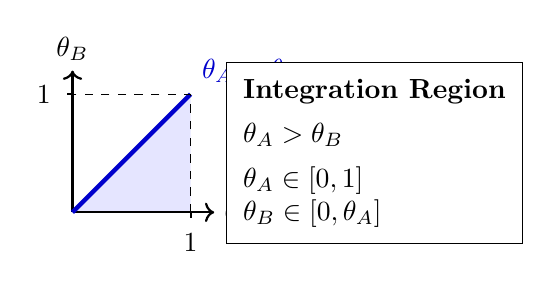
\begin{tikzpicture}[scale=1.5]
    % Background fill for the integration region
    \fill[blue!10] (0,0) -- (1,0) -- (1,1) -- cycle;
    
    % Axes
    \draw[thick, ->] (0,0) -- (1.2,0) node[right] {$\theta_A$};
    \draw[thick, ->] (0,0) -- (0,1.2) node[above] {$\theta_B$};
    
    % Line theta_A = theta_B
    \draw[ultra thick, blue!80!black] (0,0) -- (1,1) node[above right] {$\theta_A = \theta_B$};
    
    % Bounding box
    \draw[dashed] (1,0) -- (1,1) -- (0,1);
    
    % Ticks
    \draw[thick] (1,0) -- (1,-0.05) node[below=2pt] {$1$};
    \draw[thick] (0,1) -- (-0.05,1) node[left=2pt] {$1$};
    
    % Legend / Annotation Node
    \node[align=left, anchor=west, draw, fill=white, inner sep=6pt] at (1.3, 0.5) {
        \textbf{Integration Region} \\[4pt]
        $\theta_A > \theta_B$ \\[4pt]
        $\theta_A \in [0, 1]$ \\
        $\theta_B \in [0, \theta_A]$
    };
\end{tikzpicture}
\end{center}
\end{proof}

\begin{proof}[Solution to Problem 22]
$R \sim \text{Beta}(2, 2) \implies f(r) = 6r(1-r) = 6r - 6r^2$.
The payout is $V = 100 \max(R - 0.5, 0)$. By LOTUS:
\begin{align*}
\E[V] &= \int_0^1 100 \max(r - 0.5, 0) (6r - 6r^2) dr = 100 \int_{0.5}^1 (r - 0.5)(6r - 6r^2) dr \\
&= 600 \int_{0.5}^1 (r^2 - r^3 - 0.5r + 0.5r^2) dr = 600 \int_{0.5}^1 (-r^3 + 1.5r^2 - 0.5r) dr \\
&= 600 \left[ -\frac{r^4}{4} + \frac{1.5r^3}{3} - \frac{0.5r^2}{2} \right]_{0.5}^1 = 600 \left[ -\frac{r^4}{4} + \frac{r^3}{2} - \frac{r^2}{4} \right]_{0.5}^1 \\
&= 600 \left( \left[ -\frac{1}{4} + \frac{1}{2} - \frac{1}{4} \right] - \left[ -\frac{0.0625}{4} + \frac{0.125}{2} - \frac{0.25}{4} \right] \right) \\
&= 600 \left( 0 - \left[ -0.015625 + 0.0625 - 0.0625 \right] \right) = 600 (0.015625) = 9.375
\end{align*}
The expected payout is $9.375$.
\end{proof}

\begin{proof}[Solution to Problem 23]
Let $Y \sim \text{Beta}(\alpha, \alpha)$. The mean is $\mu = \frac{\alpha}{2\alpha} = 0.5$.
The variance is $\sigma^2 = \frac{\alpha^2}{(2\alpha)^2(2\alpha+1)} = \frac{1}{4(2\alpha+1)}$.
As $\alpha \to \infty$, $\sigma^2 \to 0$.
By Chebyshev's Inequality, for any $\epsilon > 0$:
\[
\Prob(|Y - 0.5| \ge \epsilon) \le \frac{\sigma^2}{\epsilon^2} = \frac{1}{4\epsilon^2(2\alpha+1)}
\]
As $\alpha \to \infty$, this probability goes to 0. Thus, the probability measure concentrates entirely at $y = 0.5$, which is the definition of weak convergence to the Dirac measure $\delta_{0.5}$.
\end{proof}

\begin{proof}[Solution to Problem 24]
$Y \sim \text{Beta}(\alpha, 1) \implies f_Y(y) = \alpha y^{\alpha-1}$ for $y \in (0, 1]$.
Let $W = -\ln(Y)$. The inverse transformation is $Y = e^{-W}$.
The Jacobian is $\left| \frac{dy}{dw} \right| = \left| -e^{-w} \right| = e^{-w}$.
The support maps from $y \in (0, 1]$ to $w \in [0, \infty)$.
\[
f_W(w) = f_Y(e^{-w}) \left| \frac{dy}{dw} \right| = \alpha (e^{-w})^{\alpha-1} e^{-w} = \alpha e^{-\alpha w + w - w} = \alpha e^{-\alpha w}
\]
This is exactly the probability density function of an Exponential distribution with rate parameter $\lambda = \alpha$.
\end{proof}

\begin{proof}[Solution to Problem 25]
$Y_1, Y_2 \sim \text{Unif}(0, 1)$. Let $Z = Y_1 Y_2$. The support of $Z$ is $(0, 1]$.
Using the product convolution formula:
\[
f_Z(z) = \int_z^1 \frac{1}{y_1} f_{Y_1}(y_1) f_{Y_2}(z/y_1) dy_1
\]
Since $f_{Y_1} = 1$ and $f_{Y_2} = 1$ within their supports, the integrand is simply $1/y_1$.
\[
f_Z(z) = \int_z^1 \frac{1}{y_1} dy_1 = \left[ \ln(y_1) \right]_z^1 = \ln(1) - \ln(z) = -\ln(z)
\]
Thus, $f_Z(z) = -\ln(z)$ for $z \in (0, 1]$.
\end{proof}

\begin{proof}[Solution to Problem 26]
\textbf{Flaw:} The student assumed $\E[Y^2] = (\E[Y])^2$. This implies the variance is zero, which is false for any continuous distribution. The expectation of a non-linear function is not the function of the expectation (Jensen's Inequality).
\textbf{Correction:} Use the raw moment formula $\E[Y^2] = \frac{\alpha(\alpha+1)}{(\alpha+\beta)(\alpha+\beta+1)}$.
For $\text{Beta}(3, 3)$: $\E[Y^2] = \frac{3(4)}{(6)(7)} = \frac{12}{42} = \frac{2}{7} \approx 0.2857$.
\end{proof}

\begin{proof}[Solution to Problem 27]
\textbf{Flaw:} The student incorrectly evaluated the Gamma function as $\Gamma(n) = n!$. The correct property is $\Gamma(n) = (n-1)!$.
\textbf{Correction:} The normalizing constant is $\frac{\Gamma(4+2)}{\Gamma(4)\Gamma(2)} = \frac{\Gamma(6)}{\Gamma(4)\Gamma(2)} = \frac{5!}{3!1!} = \frac{120}{6 \cdot 1} = 20$.
\end{proof}

\begin{proof}[Solution to Problem 28]
\textbf{Flaw:} The student assumed $\text{Var}(Y_1 + Y_2) = \text{Var}(Y_1) + \text{Var}(Y_2)$. This linearity of variance ONLY holds if $Y_1$ and $Y_2$ are strictly independent (i.e., their covariance is zero). The problem states they are "sequential batches," which strongly implies potential time-series correlation. The covariance term $2\text{Cov}(Y_1, Y_2)$ is missing.
\end{proof}

\begin{proof}[Solution to Problem 29]
\textbf{Flaw:} The student ignored the indicator function $\mathbf{1}_{[0,1]}(y)$ that defines the strict support of the Beta distribution. Integrating from $-\infty$ to $\infty$ without splitting the integral or applying the indicator is a severe measure-theoretic error. Furthermore, the substitution $u = 1-y$ flips the bounds of integration (from $[0, 1]$ to $[1, 0]$), which requires a negative sign to flip back. The student ignored both the bounds and the sign change.
\end{proof}

\begin{proof}[Solution to Problem 30]
\textbf{Flaw:} The student claimed $\text{Var}(Y^2 + Y) = \text{Var}(Y^2) + \text{Var}(Y)$. This is completely false because $Y$ and $Y^2$ are perfectly dependent random variables. The correct formula requires the covariance: $\text{Var}(Y^2 + Y) = \text{Var}(Y^2) + \text{Var}(Y) + 2\text{Cov}(Y^2, Y)$.
\end{proof}

\newpage
\section{Concept Checklist \& Question Mapping (Repeated)}

\renewcommand{\arraystretch}{1.5}
\noindent
\begin{tabularx}{\textwidth}{l X l}
\toprule
\textbf{ID} & \textbf{Theoretical Concept / Proof Technique} & \textbf{Problem Numbers} \\
\midrule
C1 & Density Normalization \& The Kernel Method & 1, 2, 3 \\
C2 & Direct Measure Computation \& Borel Set Integration & 4, 5, 6 \\
C3 & Transformations \& Expectations (LOTUS) & 7, 8, 9, 10 \\
C4 & Theoretical Parameter Proofs \& Gamma Recursion & 11, 12, 13, 14 \\
C5 & The Four-Parameter (Generalized) Beta Distribution & 15, 16, 17 \\
C6 & Bayesian Inference, Conjugacy, \& Posterior Updating & 18, 19, 20 \\
C7 & Advanced Applications: ML \& Algorithmic Trading & 21, 22, 23 \\
C8 & Measure-Theoretic Limits \& Asymptotic Behavior & 24, 25 \\
C9 & Diagnostic Testing: "Find the Flaw" (Logic/Syntax) & 26, 27, 28, 29, 30 \\
\bottomrule
\end{tabularx}

\end{document}